% Provenance (never printed): see sources/outline_sources.md (Year 1: elastic rebound and the
% seismic cycle; seismic moment and magnitudes; focal mechanisms; geodetic measurement of
% active deformation; the Gutenberg--Richter law). Exercise and problem values in the Book 3
% scratch calculator calc/ch18.py; figure data from figdata/bachelor-1/gutenberg_richter.py,
% beachballs.py and interseismic.py. Focus, epicentre, magnitude, intensity and seismometer
% are owned by Book 1 g7 (magnitude re-founded here as the moment magnitude); P and S waves by
% Book 2 g11; fault types and rake by ch. 17; stress, Coulomb and the seismogenic layer by
% ch. 16; the shear modulus by physics. Radar interferometry and the stereographic projection
% belong to later volumes (told, not defined).
\chapter{地震源}\label{ch:b1:earthquake-source}

% ledger: pp1515:1906, reid:1910
1906 年 4 月 18 日清晨，旧金山南北两侧的地面
沿一条长逾四百千米的线断裂。道路、栅栏和
横穿这条线的成排树木也被切断，每一段的两半
相距数米，西侧的一半总是向北错开。测量人员
在此前的半个世纪里曾多次测定该地区地标的位置，
地标被重新测量时，
比较结果显示的情况比断裂本身更为奇特：地面
在地震发生前的几十年间一直缓慢而平滑地弯曲，
而地震使它弹了回去。本章沿着一次地震的发展过程，从
断层的缓慢加载，到断层滑动的短短几分钟，
再由地震波和地面运动反推滑动的情况：滑动有多大，
朝哪个方向运动，下一次地震正在以多快的速度孕育，
以及各种大小的地震多久发生一次。

\begin{recall}
震源是地震破裂开始的点，其
正上方地表的点为震中；震级衡量地震的大小，
烈度衡量某地的震动强弱；地震仪以
地震图的形式记录地面运动（见第 1 册七年级）。P 波是
压缩波，最先到达，S 波是剪切波，随后到达（见第 2 册十一年级）。
断层有\omterm{def:b1:faults-folds-fabrics:fault-elements}{上盘}和\omterm{def:b1:faults-folds-fabrics:fault-elements}{下盘}；\omterm{def:b1:faults-folds-fabrics:fault-elements}{滑动矢量}
是\omterm{def:b1:faults-folds-fabrics:fault-elements}{上盘}相对于\omterm{def:b1:faults-folds-fabrics:fault-elements}{下盘}的位移，其\omterm{def:b1:faults-folds-fabrics:fault-elements}{侧伏角}
$r$ 在断层面上从\omterm{def:b1:geological-maps:attitude}{走向}量起，\omterm{def:b1:faults-folds-fabrics:fault-elements}{侧伏角}决定
断层类型：约 \ang{90} 为\omterm{def:b1:faults-folds-fabrics:fault-types}{逆断层}，约 \ang{-90} 为\omterm{def:b1:faults-folds-fabrics:fault-types}{正断层}，约 0 为\omterm{def:b1:faults-folds-fabrics:fault-types}{左行}，约
\ang{180} 为\omterm{def:b1:faults-folds-fabrics:fault-types}{右行}（见\cref{ch:b1:faults-folds-fabrics}）。弹性固体
在去除应力后恢复原状；剪切模量 $\mu$
把切应力与它产生的\omterm{def:b1:stress-strain-rheology:strain}{剪应变}联系起来（见物理学）；断层
在切应力达到其摩擦强度时滑动，地震
发生在脆性的上部\omterm{def:b1:layered-earth:layers}{地壳}，即\omterm{def:b1:stress-strain-rheology:strength-envelope}{孕震层}
（见\cref{ch:b1:stress-strain-rheology}）。长期运行的卫星定位台站
其多年记录的每日位置给出该处地面的速度，
用来测量板块的运动（见\cref{ch:b1:plate-kinematics}）。
\end{recall}

\section{弹性回跳与地震周期}\label{sec:b1:earthquake-source:cycle}

沿断层以稳定速率相互错动的两个板块，一般来说，
并不会沿它们之间的断层平稳地滑动。摩擦使断层锁定，
而远离断层的板块仍在继续运动，于是断层两侧的岩石
像弹簧一样被弯曲。当断层上的切应力达到其强度时，
断层在几秒或几分钟内滑动，弯曲的岩石随之弹回。

\begin{definition}[弹性回跳、地震周期、复发间隔]\label{def:b1:earthquake-source:seismic-cycle}
\emph{弹性回跳}\index{弹性回跳}是指断层两侧的岩石在断层被锁定、
处于应变状态时，因断层在地震中滑动而突然回复到其无应变形状的过程；
它们所储存的弹性能部分以地震波的形式释放。
断层段的\emph{地震周期}\index{地震周期}是一个反复出现的序列：
先是较长的震间阶段，在此阶段该段被锁定，周围的应变不断积累；
接着是同震阶段，即地震本身，断层在此阶段滑动；
最后是历时数月至数十年的震后阶段，
在此阶段周围介质调整到新的状态。
断层段的\emph{复发间隔}\index{复发间隔}是该段上
两次相邻大地震
之间的时间间隔。
\end{definition}
% ledger: usgs:gloss-rebound, reid:1910, usgs:pp1515-thatcher

\begin{omfigure}
\begin{tikzpicture}[>={Stealth[length=5pt]}, font=\small]
% map view of a fence across a locked dextral strike-slip fault (north up): (a) built straight;
% (b) after decades of loading, bent with the interseismic profile v(x) = -(s/pi) arctan(x/D)
% (dextral: the east side moves south); (c) after the earthquake, straight again on each side and
% offset by s at the fault. Panel 3.4 cm wide (x from -1.7 to 1.7 cm), D = 0.35 cm, s = 0.9 cm.
\def\s{0.9}\def\Dl{0.35}
\foreach \k/\t in {0/{(a) 修建围栏}, 1/{(b) 数十年的加载}, 2/{(c) 地震之后}} {
  \begin{scope}[xshift=\k*4.6cm]
    \fill[omLithSand!25] (-1.7,-1.6) rectangle (1.7,1.6);
    \draw[black!50, line width=0.4pt] (-1.7,-1.6) rectangle (1.7,1.6);
    \draw[fault, line width=1.1pt] (0,-1.6) -- (0,1.6);
    \node[anchor=north, align=center, font=\scriptsize] at (0,-1.7) {\t};
    % far-field motion of the two blocks, relative to the fault
    \draw[->, omThm, line width=0.8pt] (-1.35,-1.25) -- (-1.35,-0.45);
    \draw[->, omThm, line width=0.8pt] (1.35,1.25) -- (1.35,0.45);
    \ifnum\k=0
      \draw[line width=1.2pt, omDef] (-1.7,0) -- (1.7,0);
    \fi
    \ifnum\k=1
      \draw[line width=1.2pt, omDef] plot[domain=-1.7:1.7, samples=81, variable=\x] (\x, {-\s/pi*atan(\x/\Dl)*pi/180});
      \draw[black!45, dashed, line width=0.4pt] (-1.7,0) -- (1.7,0);
    \fi
    \ifnum\k=2
      \draw[line width=1.2pt, omDef] (-1.7,{\s/2}) -- (0,{\s/2});
      \draw[line width=1.2pt, omDef] (0,{-\s/2}) -- (1.7,{-\s/2});
      \draw[black!45, dashed, line width=0.4pt] (-1.7,0) -- (1.7,0);
      \draw[<->, line width=0.5pt] (0.18,{\s/2}) -- (0.18,{-\s/2});
      \node[anchor=west, font=\scriptsize] at (0.2,0.12) {滑动};
    \fi
  \end{scope}
}
\node[anchor=south, font=\scriptsize] at (0,1.62) {断层};
\draw[->, line width=0.5pt] (-1.5,0.75) -- (-1.5,1.15) node[above, font=\scriptsize, inner sep=1pt] {北};
\end{tikzpicture}
\par\smallskip{\small 从上方看到的\omterm{def:b1:earthquake-source:seismic-cycle}{弹性回跳}，栅栏（蓝色）
笔直建成，横跨一条锁定的\omterm{def:b1:faults-folds-fabrics:fault-types}{右行}\omterm{def:b1:faults-folds-fabrics:fault-types}{走滑断层}。红色箭头：远离断层的两个断块
相对于断层的运动。（b）断层锁定期间，
远处地面移动，栅栏随之弯曲，其形状与
\cref{sec:b1:earthquake-source:geodesy}中的震间剖面一致。（c）地震
释放了弯曲：栅栏的每一半重新变直，
两半在断层处因滑动而错开。图中的弯曲
被夸大了：实际栅栏在数十千米的范围内只弯曲几米。}
\label{fig:b1:earthquake-source:rebound}
\end{omfigure}

若断层在两次地震之间处于锁定状态，且每次地震都抵消了
自上次地震以来板块累积的错动，则板块运动决定了
该循环的节奏。

\begin{proposition}[由滑动速率得复发间隔]\label{prop:b1:earthquake-source:recurrence}
设某段断层以长期滑动速率 $\dot s$ 加载，
两次地震之间处于锁定状态，且每次地震的滑动量均为 $D$。则
其地震的\omterm{def:b1:earthquake-source:seismic-cycle}{复发间隔}为
\[
  T = \frac{D}{\dot s} .
\]
若仅有滑动速率的分数 $c$ 被锁定，其余部分
在无地震的情况下稳定滑动，则 $T = D/(c\,\dot s)$。
\end{proposition}

\begin{proof}
在长时间 $t$ 内，断层两侧彼此相对移动
$\dot s\,t$。远离断层处地面稳定移动，因此在断层本身
断层本身的同等位移须仅由地震补足：若
$N$ 次地震在时间 $t$ 内发生，则 $N D = \dot s\,t$，至多相差
一次地震的滑动量，且 $t/N \to D/\dot s$。若滑动的分数 $1-c$ 以稳定滑动完成，
则地震补足 $c\,\dot s\,t$，于是
$t/N \to D/(c\,\dot s)$。
\end{proof}

以圣安德烈亚斯断层的典型数值为例，每次大地震的滑动量为 \qty{4}{m}，
滑动速率为 \qty{20}{mm.\text{年}^{-1}}，则\omterm{def:b1:earthquake-source:seismic-cycle}{复发间隔}为
\qty{200}{\text{年}}。在加利福尼亚州中部的沃勒斯溪，一条横穿断层的溪流河道
自切割以来，已被错开 \qty{128}{m}，历时 \num{3587} 年，
平均速率为 \qty{36}{mm.\text{年}^{-1}}，接近该处其他错距上测得的
约 \qty{34}{mm.\text{年}^{-1}}。该段上一次大地震
发生于 1857 年，滑动量近 \qty{10}{m}，按此速率累积这些位移约需
三个世纪。
% ledger: usgs:pp1515-thatcher, usgs:pp1515-wallace, commons:wallace-creek

\begin{omfigure}
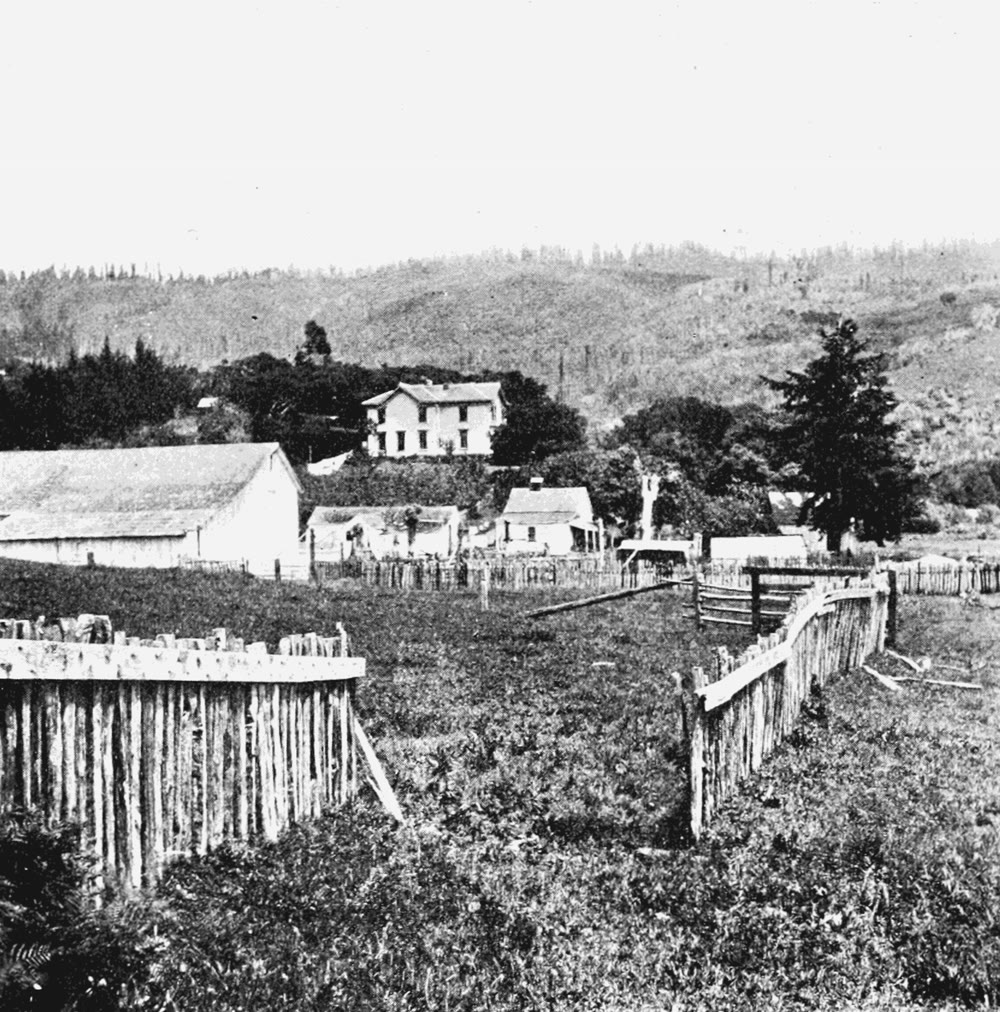
\includegraphics[height=5.6cm]{images/book3/b1-fence-1906.jpg}\hfill
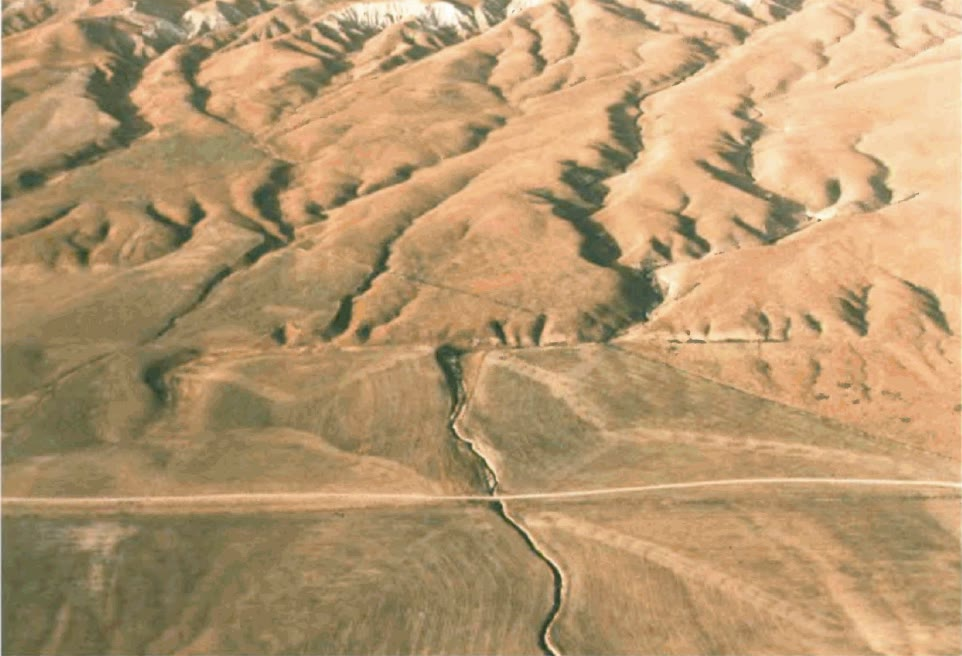
\includegraphics[height=5.6cm]{images/book3/b1-wallace-creek.jpg}
\par\smallskip{\small 左：旧金山以北马林县农田中的栅栏，
被 1906 年的破裂所穿过，照片发表于同年的文章“地震断层使土地
分离”。照片取自 \emph{Popular Science
Monthly}，第 69 卷（1906 年），公有领域。右：卡里佐平原的沃勒斯溪，
从空中俯瞰：溪流自丘陵（上方）流下，并在丘陵脚下
与圣安德烈亚斯断层相交，河道在此向侧方错开
\qty{130}{m}，这一错距是数千年地震累积的结果。
照片：
R.~E.~华莱士，美国地质调查局，公有领域。两图均取自维基
共享资源。}
\label{fig:b1:earthquake-source:offsets}
\end{omfigure}
% ledger: commons:psm-fence, commons:wallace-creek

该命题给出的是平均值，而非时间表。在同一断层的帕克菲尔德附近，
1857 年发生了一次震级约为 6 的地震，此后又接连发生了五次
性质相近的地震，发生于同一约 \qty{30}{km} 的段落上，间隔近 22 年，
直至 1966 年；下一次地震原本预计在 1993 年之前发生，
实际却于 2004 年到来，\omterm{def:b1:earthquake-source:mw}{矩震级}为 6.0，事前没有任何明显的预警迹象。
断层的强度、每次地震的滑动量以及相邻断层段施加的加载，
都会在不同循环之间发生变化，因此
\omterm{def:b1:earthquake-source:seismic-cycle}{地震周期}用平均\omterm{def:b1:earthquake-source:seismic-cycle}{复发间隔}及其离散程度来描述，比用一个
固定周期更为恰当。
% ledger: pp1515:parkfield, bl85:parkfield, usgs:hist-mw, bakun:2005

有些断层段根本不会锁定。在帕克菲尔德与
圣胡安巴蒂斯塔之间，圣安德烈亚斯断层的中段发生蠕滑：断层上的稳定滑动
几乎承担了板块运动的全部，两侧即使有应变积累也很少，
因此该段没有大地震；1857 年的大破裂始于其南端，
而 1906 年的破裂则止于其北端。
在其部分区域发生蠕滑的断层，只是部分被锁定，
这正是命题中的系数 $c$。
% ledger: pp1515:creep, pp1515:1906

\begin{inthefield}[通过探槽读取过去的地震]
仪器记录地震的历史仅有一个多世纪，远不及
大多数断层的一个循环。古地震学者通过读取大地来延长记录。
在一条活动断层上横向挖掘一条深数米的探槽，
该处曾在沼泽、湖泊
或小型冲积扇中连续沉积多层沉积物。探槽壁上，每次地震都表现为被断层切割并错开的岩层，
又被较新的沉积物完整覆盖；被后期沉积物掩埋的陡坎；
曾液化并沿裂隙上涌、铺展于当时地表之上的砂层。
紧邻每一断裂下方和上方地层中的泥炭或植物残体，
经放射性碳测年，由此限定每次地震的年代：
圣安德烈亚斯断层上的一处沼泽保存了十二次地震的记录。
沿海岸地带，由海啸沉积的砂层，以及因地震骤然下沉约一米的沼泽，
随后被潮汐泥掩埋，记录了大型俯冲型地震。
在圣安德烈亚斯断层上，历史时期的大部分滑动都伴随着
震级为 6 或更大的地震。
\end{inthefield}
% ledger: pp1515:pallett, atwater:1987

\begin{history}[哈里·菲尔丁·赖德与弹性回跳]
哈里·菲尔丁·赖德是一位美国物理学家，曾任州委员会成员，
该委员会研究 1906 年的地震。他比较了各点的位置，
这些点于 1851--1865 年、1874--1892 年及地震之后测得，他
发现自第一次测量以来，圣安德烈亚斯断层两侧较远的各点已
相对移动约 \qty{3.2}{m}，略多于
断层上约 \qty{6}{m} 滑动量的一半：在地震前半个世纪，
导致断层破裂的应变已积累了一半。只有
弹性力才能使大地如此突然地移动，他将这种
突然的回复称为\omterm{def:b1:earthquake-source:seismic-cycle}{弹性回跳}。他于 1910 年在委员会报告的第二卷中发表了这一成果，
它至今仍是\omterm{def:b1:earthquake-source:seismic-cycle}{地震周期}的主要模型。
此后，卫星定位已测得他只能推断的
弯曲。
\end{history}
% ledger: reid:1910, pp1515:1906

\section{地震矩与震级}\label{sec:b1:earthquake-source:moment}

地震的大小由其滑动量、
发生滑动的断层面积决定，并以岩石的刚度加权。

\begin{definition}[地震矩]\label{def:b1:earthquake-source:moment}
设地震平均滑动量为 $D$，破裂面面积为 $A$，
岩石的剪切模量为 $\mu$（该字母也表示一个摩擦因数，
见\cref{ch:b1:stress-strain-rheology}，由上下文判断其含义）。其\emph{地震矩}\index{地震矩}
为
\[
  M_0 = \mu A D ,
\]
单位为牛顿·米。
\end{definition}
% ledger: usgs:gloss-moment

其单位与力矩相同。断层上的一次滑动所发出的波，与
作用于震源处的两对反向力（即两个力偶）所发出的波相同，而\omterm{def:b1:earthquake-source:moment}{地震矩}
即每个力偶的力矩（这一等价关系，即双力偶，在本科三年级分册中
证明）。该力矩的量纲与能量相同，但它并不是能量：
以波的形式辐射出的能量只占其中一小部分。对于
\omterm{def:b1:layered-earth:layers}{地壳}岩石，取 $\mu$ 为 \qty{30}{GPa}。
% ledger: kanamori:1977, sk:mu-locking

如今，\omterm{def:b1:earthquake-source:moment}{地震矩}由全球各地记录的长周期波算得。
对于 2011 年 3 月 11 日的东北地震，美国地质调查局的首选解给出
$M_0 = \qty{5.59e22}{N.m}$。断层的滑动区域
长约 \qty{400}{km}、宽约 \qty{150}{km}，由定义
可得平均滑动量
\[
  D = \frac{M_0}{\mu A}
    = \frac{\num{5.59e22}}{\num{3e10}\times\num{4e5}\times\num{1.5e5}}
    \approx \qty{31}{m} ,
\]
而破裂模型表明，其位移最大的部分可达
\qtyrange{50}{60}{m}。
% ledger: usgs:tohoku-mt, usgs:tohoku-summary

第 1 册中的震级，是根据地震图上的
波的振幅算出的。这类震级只测量某一周期的波，一旦破裂
长度远大于这些波的波长（约几至五十千米）时，
振幅便不再随破裂大小增长，震级趋于饱和。
体波震级在 6.5 附近饱和，面波震级在 8.3 附近饱和。
2011 年东北地震的首次海啸预警，依据的是这类
震级，但这类震级对 8 级或更大的地震并不适用，它
低估了地震波。\omterm{def:b1:earthquake-source:moment}{地震矩}不会饱和，震级因此
改由\omterm{def:b1:earthquake-source:moment}{地震矩}定义。
% ledger: kanamori:1977, usgs:magtypes, jma:warning

\begin{definition}[矩震级]\label{def:b1:earthquake-source:mw}
地震的\emph{矩震级}\index{矩震级}，由其\omterm{def:b1:earthquake-source:moment}{地震矩}
$M_0$（以牛顿·米为单位）确定，为
\[
  M_w = \tfrac23\left(\log_{10} M_0 - 9.1\right) .
\]
\end{definition}
% ledger: usgs:magtypes

托马斯·汉克斯与金森博史于 1979 年定义了该标度，常数取
9.05 而非 9.1，二者在 $M_w$ 上相差 0.03；常数的选取
旨在与较旧震级在未饱和处相符。第 1 册中的
震级对大地震即为此数：对于东北地震，
$M_w = \tfrac23(\log_{10}\num{5.59e22} - 9.1) = \tfrac23(22.75 - 9.1) = 9.1$;
1960 年智利大地震与 1964 年阿拉斯加地震的
\omterm{def:b1:earthquake-source:mw}{矩震级}分别为 9.5 与 9.2，这是较旧震级无法
体现的量级。
% ledger: hk:1979, kanamori:1977, usgs:hist-mw, usgs:tohoku-mt

\begin{proposition}[震级的一个单位]\label{prop:b1:earthquake-source:moment-steps}
\omterm{def:b1:earthquake-source:moment}{地震矩}为 $M_0 = 10^{1.5 M_w + 9.1}$ 牛顿·米。\omterm{def:b1:earthquake-source:mw}{矩震级}每增加
一个单位，\omterm{def:b1:earthquake-source:moment}{地震矩}便乘以 $10^{1.5} \approx 31.6$，增加两个单位则乘以
$1000$。若辐射能量为\omterm{def:b1:earthquake-source:moment}{地震矩}的固定比例，则它
也按相同比例增长。
\end{proposition}

\begin{proof}
由定义解出 $M_0$，得 $\log_{10} M_0 = 1.5 M_w + 9.1$，
对两次地震有
\[
  \log_{10}\frac{M_0'}{M_0} = 1.5\,(M_w' - M_w) ,
\]
即一个单位时为 $1.5$，两个单位时为 $3$。若辐射能量 $E_s = k M_0$，
两次地震中 $k$ 相同，则 $E_s'/E_s = M_0'/M_0$。
\end{proof}

金森近似 $E_s \approx M_0/(2\times10^4)$（在本阶段不加证明地承认），是
上一句的假设；震级每增加一个单位，能量约增大 32 倍，
第 1 册中所见的此因子，正是本命题。由于 $M_0 = \mu A D$，且
地震的滑动量随破裂尺度增大，因此大震级
需要大的断层。1906 年的破裂长约 \qty{430}{km}，
使\omterm{def:b1:stress-strain-rheology:strength-envelope}{孕震层}破裂至约 \qty{15}{km} 深，平均滑动量为几米：
取 $D = \qty{4}{m}$，$M_0 = \num{3e10}\times\num{4.3e5}\times\num{1.5e4}
\times 4 = \qty{7.7e20}{N.m}$，$M_w = 7.9$，即目录所列的震级。
震级 9 的地震需要长达数百千米、
宽逾一百千米的破裂面，这只有俯冲带
中\omterm{def:b1:geological-maps:attitude}{倾角}平缓的界面才能提供。
% ledger: kanamori:1977, pp1515:1906, usgs:hist-mw, usgs:pp1515-thatcher

\section{震源机制}\label{sec:b1:earthquake-source:focal}

P 波是最先到达地震仪的波。其\omterm{def:b1:earthquake-source:focal-mechanism}{初动}，即
竖直记录上的第一次摆动，波以推的方式到达时向上，
即地面受压并被抛离震源；而波以拉的方式到达时则
向下。围绕地震，推与拉按某种图样排列，
这一图样给出了断层的方位与滑动方向。

\begin{proposition}[初动的符号]\label{prop:b1:earthquake-source:first-motion}
设向上法向为 $\mathbf n$ 的断层，沿单位矢量 $\mathbf d$ 滑动
（即\omterm{def:b1:faults-folds-fabrics:fault-elements}{上盘}相对于\omterm{def:b1:faults-folds-fabrics:fault-elements}{下盘}的滑动）。自震源出发的
P 波沿单位方向 $\mathbf x$ 传播，若
$(\mathbf n\cdot\mathbf x)(\mathbf d\cdot\mathbf x) > 0$ 则以推的形式到达，而若
$(\mathbf n\cdot\mathbf x)(\mathbf d\cdot\mathbf x) < 0$ 则以拉的形式到达。推与拉
因此分布于四个象限，它们由断层面
（$\mathbf n\cdot\mathbf x = 0$）以及与滑动方向垂直的平面
（$\mathbf d\cdot\mathbf x = 0$）隔开。
\end{proposition}

\begin{proof}
当 $\mathbf n\cdot\mathbf x > 0$ 时，方向指向\omterm{def:b1:faults-folds-fabrics:fault-elements}{上盘}，
\omterm{def:b1:faults-folds-fabrics:fault-elements}{上盘}相对\omterm{def:b1:faults-folds-fabrics:fault-elements}{下盘}沿 $\mathbf d$ 移动：前方的岩石
（$\mathbf d\cdot\mathbf x > 0$）受压，后方的岩石
（$\mathbf d\cdot\mathbf x < 0$）受拉。
当 $\mathbf n\cdot\mathbf x < 0$ 时，方向指向\omterm{def:b1:faults-folds-fabrics:fault-elements}{下盘}，
\omterm{def:b1:faults-folds-fabrics:fault-elements}{下盘}相对\omterm{def:b1:faults-folds-fabrics:fault-elements}{上盘}沿 $-\mathbf d$ 移动，故符号相反。两种情形下，
\omterm{def:b1:earthquake-source:focal-mechanism}{初动}的符号均与 $(\mathbf n\cdot\mathbf x)(\mathbf
d\cdot\mathbf x)$ 相同。
\end{proof}

上述论证只给出符号。\omterm{def:b1:earthquake-source:focal-mechanism}{初动}的振幅与
$2(\mathbf n\cdot\mathbf x)(\mathbf d\cdot\mathbf x)$ 成正比，因而
在距两个\omterm{def:b1:earthquake-source:focal-mechanism}{节面}均为 \ang{45} 的方向上最大，在\omterm{def:b1:earthquake-source:focal-mechanism}{节面}上为零，此处
不加证明地承认（见本科三年级分册）。

\begin{omfigure}
\begin{tikzpicture}[>={Stealth[length=5pt]}, font=\small, scale=0.95]
% map view around a vertical dextral fault striking north, the focus at the origin, rays leaving
% horizontally: pushes where (n.x)(d.x) > 0, i.e. in the NW and SE quadrants (beachballs.py,
% first_motion(0, 90, 180, x)). Stations at 20 azimuths on a circle of radius 2.3.
\fill[omThm!22] (0,0) -- (0,2.8) arc[start angle=90, end angle=180, radius=2.8] -- cycle;
\fill[omThm!22] (0,0) -- (0,-2.8) arc[start angle=270, end angle=360, radius=2.8] -- cycle;
\draw[black!40, line width=0.4pt] (0,0) circle[radius=2.8];
\draw[fault, line width=1.3pt] (0,-3.1) -- (0,3.1) node[above, font=\scriptsize] {断层（节面）};
\draw[black, dashed, line width=0.7pt] (-3.1,0) -- (3.1,0) node[right, font=\scriptsize, align=left] {辅助面};
% slip: the west block moves north, the east block south
\draw[->, line width=1pt] (-0.3,-0.8) -- (-0.3,0.8);
\draw[->, line width=1pt] (0.3,0.8) -- (0.3,-0.8);
% stations
\foreach \a in {9,27,...,351} {
  \pgfmathsetmacro{\fm}{-sin(\a)*cos(\a)}  % (n.x)(d.x) with n = east, d = south, x = (sin a, cos a)
  \pgfmathparse{\fm>0 ? 1 : 0}
  \ifnum\pgfmathresult=1
    \fill[black] ({2.3*sin(\a)},{2.3*cos(\a)}) circle[radius=0.11];
  \else
    \draw[black, fill=white, line width=0.6pt] ({2.3*sin(\a)},{2.3*cos(\a)}) circle[radius=0.11];
  \fi
}
% P and T axes
\draw[<-, omProp, line width=1.1pt] ({0.7*sin(45)},{0.7*cos(45)}) -- ({1.6*sin(45)},{1.6*cos(45)}) node[above right, font=\scriptsize, inner sep=1pt] {P};
\draw[<-, omProp, line width=1.1pt] ({0.7*sin(225)},{0.7*cos(225)}) -- ({1.6*sin(225)},{1.6*cos(225)});
\draw[->, omProp, line width=1.1pt] ({0.7*sin(315)},{0.7*cos(315)}) -- ({1.6*sin(315)},{1.6*cos(315)}) node[above left, font=\scriptsize, inner sep=1pt] {T};
\draw[->, omProp, line width=1.1pt] ({0.7*sin(135)},{0.7*cos(135)}) -- ({1.6*sin(135)},{1.6*cos(135)});
\fill (0,0) circle[radius=0.06];
% legend
\begin{scope}[xshift=4.6cm, yshift=2.4cm]
  \fill[black] (0,0) circle[radius=0.11]; \node[anchor=west, font=\scriptsize] at (0.2,0) {推：初动向上};
  \draw[black, fill=white, line width=0.6pt] (0,-0.5) circle[radius=0.11]; \node[anchor=west, font=\scriptsize] at (0.2,-0.5) {拉：初动向下};
  \fill[omThm!22] (-0.12,-1.12) rectangle (0.12,-0.88); \node[anchor=west, font=\scriptsize] at (0.2,-1.0) {推的象限};
  \draw[->] (-0.1,-1.6) -- (-0.1,-1.25); \node[anchor=west, font=\scriptsize] at (0.2,-1.42) {北};
\end{scope}
\end{tikzpicture}
\par\smallskip{\small 竖直\omterm{def:b1:faults-folds-fabrics:fault-types}{右行}\omterm{def:b1:faults-folds-fabrics:fault-types}{走滑断层}（\omterm{def:b1:geological-maps:attitude}{走向}为南北向）周围的\omterm{def:b1:earthquake-source:focal-mechanism}{初动}，俯视图，
波从震源水平射出，射向周围各方向的台站。黑色箭头为两侧岩块的滑动方向。
推的象限位于西北与东南两个象限，
拉的象限位于另外两个象限；断层与\omterm{def:b1:earthquake-source:focal-mechanism}{辅助面}将它们分隔开。
\omterm{def:b1:earthquake-source:focal-mechanism}{P 轴}（箭头指向内）平分拉的象限，
\omterm{def:b1:earthquake-source:focal-mechanism}{T 轴}（箭头指向外）平分推的象限。若沿虚线所示平面发生\omterm{def:b1:faults-folds-fabrics:fault-types}{左行}滑动，
且该平面南侧岩块向东移动，
则会得到完全相同的图样
（见\cref{prop:b1:earthquake-source:auxiliary}）。}
\label{fig:b1:earthquake-source:quadrants}
\end{omfigure}

乘积 $(\mathbf n\cdot\mathbf x)(\mathbf d\cdot\mathbf x)$ 在
交换 $\mathbf n$ 与 $\mathbf d$ 时不变。这一对称性是
\omterm{def:b1:earthquake-source:focal-mechanism}{震源机制}的核心事实。

\begin{definition}[震源机制、节面、辅助面、P 轴、T 轴]\label{def:b1:earthquake-source:focal-mechanism}
地震仪记录到的 P 波的\emph{初动}\index{初动}，是
竖直记录上地面最初运动的方向，向上或向下。
地震的\emph{震源机制}\index{震源机制}，是
断层面的方位及其上的滑动方向，由地震波求得。
经过震源、把推与拉分隔开的两个相互垂直的平面，
称为其\emph{节面}\index{节面}；其一是断层面，
另一个与滑动方向垂直，即\emph{辅助面}\index{辅助面}。
\emph{P 轴}\index{P 轴}与\emph{T 轴}\index{T 轴}是距两个节面均为
\ang{45} 的方向，
分别位于拉象限与推象限
的中线上：
\[
  \mathbf P = \frac{\mathbf n - \mathbf d}{\sqrt2}, \qquad
  \mathbf T = \frac{\mathbf n + \mathbf d}{\sqrt2} .
\]
\end{definition}
% ledger: yvo:beachball, usgs:gloss-moment

\begin{proposition}[两个节面]\label{prop:b1:earthquake-source:auxiliary}
滑动 $\mathbf d$ 发生在法向为 $\mathbf n$ 的平面上，与滑动
$\mathbf n$ 发生在法向为 $\mathbf d$ 的平面上，在每个方向上给出相同的\omterm{def:b1:earthquake-source:focal-mechanism}{初动}。
因此，\omterm{def:b1:earthquake-source:focal-mechanism}{初动}可以确定两个\omterm{def:b1:earthquake-source:focal-mechanism}{节面}、\omterm{def:b1:earthquake-source:focal-mechanism}{P 轴}与 \omterm{def:b1:earthquake-source:focal-mechanism}{T 轴}，
以及每个\omterm{def:b1:earthquake-source:focal-mechanism}{节面}上的滑动方向，但无法判断哪一个\omterm{def:b1:earthquake-source:focal-mechanism}{节面}是
断层面。
\end{proposition}

\begin{proof}
$(\mathbf n\cdot\mathbf x)(\mathbf d\cdot\mathbf x)$ 的符号在交换
$\mathbf n$ 与 $\mathbf d$ 时不变；平面
$\mathbf n\cdot\mathbf x = 0$ 与 $\mathbf d\cdot\mathbf x = 0$ 互换，
$\mathbf n \pm \mathbf d$ 不变。数对 $(\mathbf n, \mathbf d)$ 与
数对 $(-\mathbf n, -\mathbf d)$ 描述的是从另一侧岩块看到的同一滑动，
二者给出的乘积也相同。\omterm{def:b1:earthquake-source:focal-mechanism}{初动}中并无
任何信息可区分这两种描述。
\end{proof}

要判断哪一个\omterm{def:b1:earthquake-source:focal-mechanism}{节面}发生了滑动，地震学家需借助其他证据：
余震沿之排列的平面、地表可见的断层，
以及地震所在的板块边界。2004 年苏门答腊–安达曼大地震的
两个\omterm{def:b1:earthquake-source:focal-mechanism}{节面}分别向东北倾斜 \ang{8} 与
向西南倾斜 \ang{83}。该地区早先的地震及板块模型均表明，下沉的板片
沿一个向东北缓倾的平面分布，因此取较浅的平面为断层面：
此次地震破裂了俯冲带的板块界面，
其余震分布范围超过
\qty{1300}{km}。
% ledger: usgs:sumatra-mt, usgs:sumatra-summary

因为 \omterm{def:b1:earthquake-source:focal-mechanism}{P 轴}位于拉力区的中部，\omterm{def:b1:earthquake-source:focal-mechanism}{T 轴}位于推力区的中部，
人们常把它们当作最大与最小压应力的方向，
即 $\sigma_1$ 与 $\sigma_3$。这只是近似。
新断层的形成角为 $\ang{45} - \phi/2$（自 $\sigma_1$ 起算），
而非 \ang{45}（见\cref{ch:b1:stress-strain-rheology}），老断层的滑动方向
则可能又有不同，因此一次地震的轴线可能与\omterm{def:b1:stress-strain-rheology:principal}{主应力}
相差数十度；一个地区的应力须由许多次地震的\omterm{def:b1:earthquake-source:focal-mechanism}{震源机制}
综合求得。

\omterm{def:b1:earthquake-source:focal-mechanism}{震源机制}定义在焦点周围的一个球面上。作图时取该球面的下半球，
每条射向远处台站的射线都穿过它，并将其投影到一个圆盘上：
对单位矢量 $\mathbf x = (E, N, U)$ 的射线（$U \le 0$），
其投影点为
\[
  (X, Y) = \frac{(E, N)}{\sqrt{1 - U}} ,
\]
圆心对应竖直方向，水平方向位于单位圆上。这种投影保持面积不变
（在本阶段不加证明地承认；球面的各种投影将在本科三年级分册中研究），
因此每个象限在圆盘上所占的面积恰为其真实份额。
推力象限涂阴影；此图称为震源球。
% ledger: yvo:beachball

\begin{omfigure}
\begin{tikzpicture}[font=\small]
% lower-hemisphere equal-area beach balls, compressional quadrants shaded (figdata/bachelor-1/beachballs.py)
\foreach \n/\c/\t/\x in {normal/2/{(a) 正断层\\ $090/60$，侧伏角 \ang{-90}}/0,
                         reverse/1/{(b) 逆断层\\ $090/30$，侧伏角 \ang{90}}/3.65,
                         strikeslip/2/{(c) 走滑断层\\ $090/90$，侧伏角 \ang{180}}/7.3,
                         tohoku/2/{(d) 东北地震，2011 年\\ $282/8$，侧伏角 \ang{78}}/10.95} {
  \begin{axis}[at={(\x cm,0)}, anchor=center, width=2.9cm, height=2.9cm, scale only axis,
      axis equal image, xmin=-1.04, xmax=1.04, ymin=-1.04, ymax=1.04, hide axis, clip=false]
    \fill[white] (axis cs:0,0) circle[radius=1];
    \addplot[fill=omThm!55, draw=none] table[x=X, y=Y] {figdata/out/bachelor-1-beachballs-\n-c1.dat};
    \ifnum\c=2
      \addplot[fill=omThm!55, draw=none] table[x=X, y=Y] {figdata/out/bachelor-1-beachballs-\n-c2.dat};
    \fi
    \addplot[black, line width=0.6pt] table[x=X, y=Y] {figdata/out/bachelor-1-beachballs-\n-p1.dat};
    \addplot[black, line width=0.6pt] table[x=X, y=Y] {figdata/out/bachelor-1-beachballs-\n-p2.dat};
    \draw[black, line width=0.8pt] (axis cs:0,0) circle[radius=1];
    \draw[black, line width=0.5pt] (axis cs:0,1) -- (axis cs:0,1.12) node[above, font=\scriptsize, inner sep=1pt] {北};
    \addplot[only marks, mark=none, nodes near coords={\textbf{P}}, nodes near coords align=center, every node near coord/.append style={font=\scriptsize, inner sep=0pt}] table[x=X, y=Y] {figdata/out/bachelor-1-beachballs-\n-P.dat};
    \addplot[only marks, mark=none, nodes near coords={\textbf{T}}, nodes near coords align=center, every node near coord/.append style={font=\scriptsize, inner sep=0pt}] table[x=X, y=Y] {figdata/out/bachelor-1-beachballs-\n-T.dat};
    \node[anchor=north, align=center, font=\scriptsize] at (axis cs:0,-1.12) {\t};
  \end{axis}
}
\end{tikzpicture}
\par\smallskip{\small 震源球：焦点周围的下半球，等积投影，北向朝上，
推力象限涂阴影，P 与 T 标出两轴（轴线靠近边缘时，字母向内移动）。
每个\omterm{def:b1:earthquake-source:focal-mechanism}{震源机制}由一个\omterm{def:b1:earthquake-source:focal-mechanism}{节面}的\omterm{def:b1:geological-maps:attitude}{产状}（\omterm{def:b1:geological-maps:attitude}{倾向}与\omterm{def:b1:geological-maps:attitude}{倾角}）
及该面上滑动的\omterm{def:b1:faults-folds-fabrics:fault-elements}{侧伏角}给出。
(a) 向东倾斜 \ang{60} 的\omterm{def:b1:faults-folds-fabrics:fault-types}{正断层}：拉力象限充满中心；
(b) 向东倾斜 \ang{30} 的\omterm{def:b1:faults-folds-fabrics:fault-types}{逆断层}：推力象限充满中心；
(c) 竖直的\omterm{def:b1:faults-folds-fabrics:fault-types}{走滑断层}：四个象限相交于中心；
(d) 2011 年东北地震（美国地质调查局矩张量）：
日本之下一个\omterm{def:b1:geological-maps:attitude}{倾角}为 \ang{8}、\omterm{def:b1:geological-maps:attitude}{倾向}为 $282$ 的逆冲面，
东侧为陡倾的\omterm{def:b1:earthquake-source:focal-mechanism}{辅助面}。}
\label{fig:b1:earthquake-source:beachballs}
\end{omfigure}
% ledger: usgs:tohoku-mt

地震学家用每个\omterm{def:b1:earthquake-source:focal-mechanism}{节面}的\omterm{def:b1:geological-maps:attitude}{走向}、\omterm{def:b1:geological-maps:attitude}{倾角}和\omterm{def:b1:faults-folds-fabrics:fault-elements}{侧伏角}来表示\omterm{def:b1:earthquake-source:focal-mechanism}{震源机制}；
\omterm{def:b1:geological-maps:attitude}{走向}为\omterm{def:b1:geological-maps:attitude}{倾向}减去 \ang{90}，
见\cref{ch:b1:faults-folds-fabrics}。对东北地震而言，两个\omterm{def:b1:earthquake-source:focal-mechanism}{节面}的
\omterm{def:b1:geological-maps:attitude}{走向}、\omterm{def:b1:geological-maps:attitude}{倾角}和\omterm{def:b1:faults-folds-fabrics:fault-elements}{侧伏角}分别为 $192/8/78$ 与 $24/81/91$，\omterm{def:b1:earthquake-source:focal-mechanism}{P 轴}与 \omterm{def:b1:earthquake-source:focal-mechanism}{T 轴}的\omterm{def:b1:field-lab-methods-1:trend-plunge}{倾伏向}
分别为 $113$ 与 $296$，\omterm{def:b1:field-lab-methods-1:trend-plunge}{倾伏角}分别为 \ang{36} 与 \ang{53}。\omterm{def:b1:earthquake-source:focal-mechanism}{辅助面}由断层面导出：
其法向为 $\mathbf d$，滑动为 $\mathbf n$。\omterm{def:b1:earthquake-source:focal-mechanism}{辅助面}的求法是：
由\omterm{def:b1:geological-maps:attitude}{走向}、\omterm{def:b1:geological-maps:attitude}{倾角}和\omterm{def:b1:faults-folds-fabrics:fault-elements}{侧伏角}算出 $\mathbf n$ 与 $\mathbf d$，
将二者互换，再反推出\omterm{def:b1:geological-maps:attitude}{走向}、\omterm{def:b1:geological-maps:attitude}{倾角}和\omterm{def:b1:faults-folds-fabrics:fault-elements}{侧伏角}，
即可得到\omterm{def:b1:earthquake-source:focal-mechanism}{辅助面}（见\cref{exo:b1:earthquake-source:7}）。
% ledger: usgs:tohoku-mt

\begin{method}[判读震源球]\label{met:b1:earthquake-source:beachball}
\begin{enumerate}
  \item 看中心，中心代表竖直方向。阴影（竖直向下的推）表示\omterm{def:b1:faults-folds-fabrics:fault-types}{逆断层}或逆冲分量；
        空白表示\omterm{def:b1:faults-folds-fabrics:fault-types}{正断层}分量。
        过中心相交的两条直线表示走滑型\omterm{def:b1:earthquake-source:focal-mechanism}{震源机制}。
  \item 找出两个\omterm{def:b1:earthquake-source:focal-mechanism}{节面}，即界定各象限的曲线。过中心的\omterm{def:b1:earthquake-source:focal-mechanism}{节面}为竖直面；
        其余\omterm{def:b1:earthquake-source:focal-mechanism}{节面}朝其曲线所在一侧倾斜，
        曲线越靠近边缘，\omterm{def:b1:geological-maps:attitude}{倾角}越
        缓。
  \item 在阴影象限中部找出 \omterm{def:b1:earthquake-source:focal-mechanism}{T 轴}，在空白象限中部找出 \omterm{def:b1:earthquake-source:focal-mechanism}{P 轴}：
        地面沿 P 方向缩短，
        沿 T 方向伸长。
  \item 对每个\omterm{def:b1:earthquake-source:focal-mechanism}{节面}，读出或算出\omterm{def:b1:faults-folds-fabrics:fault-elements}{侧伏角}，并
        由\cref{def:b1:faults-folds-fabrics:fault-types}判定其为何种断层。两个\omterm{def:b1:earthquake-source:focal-mechanism}{节面}的
        倾滑性质（正断或逆断）总是相同，而走滑性质相反：
        走滑型\omterm{def:b1:earthquake-source:focal-mechanism}{震源机制}给出一个\omterm{def:b1:faults-folds-fabrics:fault-types}{右行}
        \omterm{def:b1:earthquake-source:focal-mechanism}{节面}和一个\omterm{def:b1:faults-folds-fabrics:fault-types}{左行}\omterm{def:b1:earthquake-source:focal-mechanism}{节面}。
  \item 依据余震、地质条件或板块边界，
        选定断层面。
\end{enumerate}
\end{method}

\begin{inthelab}[在地震台站]
\begin{minipage}[t]{0.6\linewidth}\vspace{0pt}
大地震发生后数分钟内，其波已被数百个台站记录，
数据几乎实时传至各观测台的分析人员。
P 波的初至，即距离越远到达台站越晚的那一波，
在记录上被拾取，用以定位震源。随后，
接下来数十分钟内记录的长周期慢波，与为试算震源计算的波形相比较；
拟合最好的震源给出矩张量，
其中包含\omterm{def:b1:earthquake-source:moment}{地震矩}、\omterm{def:b1:earthquake-source:mw}{矩震级}和两个\omterm{def:b1:earthquake-source:focal-mechanism}{节面}，
三者一并给出。对于较小的地震，信号太弱，无法如此处理，分析人员
便读取最近台站记录上的\omterm{def:b1:earthquake-source:focal-mechanism}{初动}，并据此拟合\omterm{def:b1:earthquake-source:focal-mechanism}{节面}，
方法即本节所述。每个解都连同其不确定度发布，
并随数据陆续到达而修订。
\end{minipage}\hfill
\begin{minipage}[t]{0.36\linewidth}\vspace{0pt}
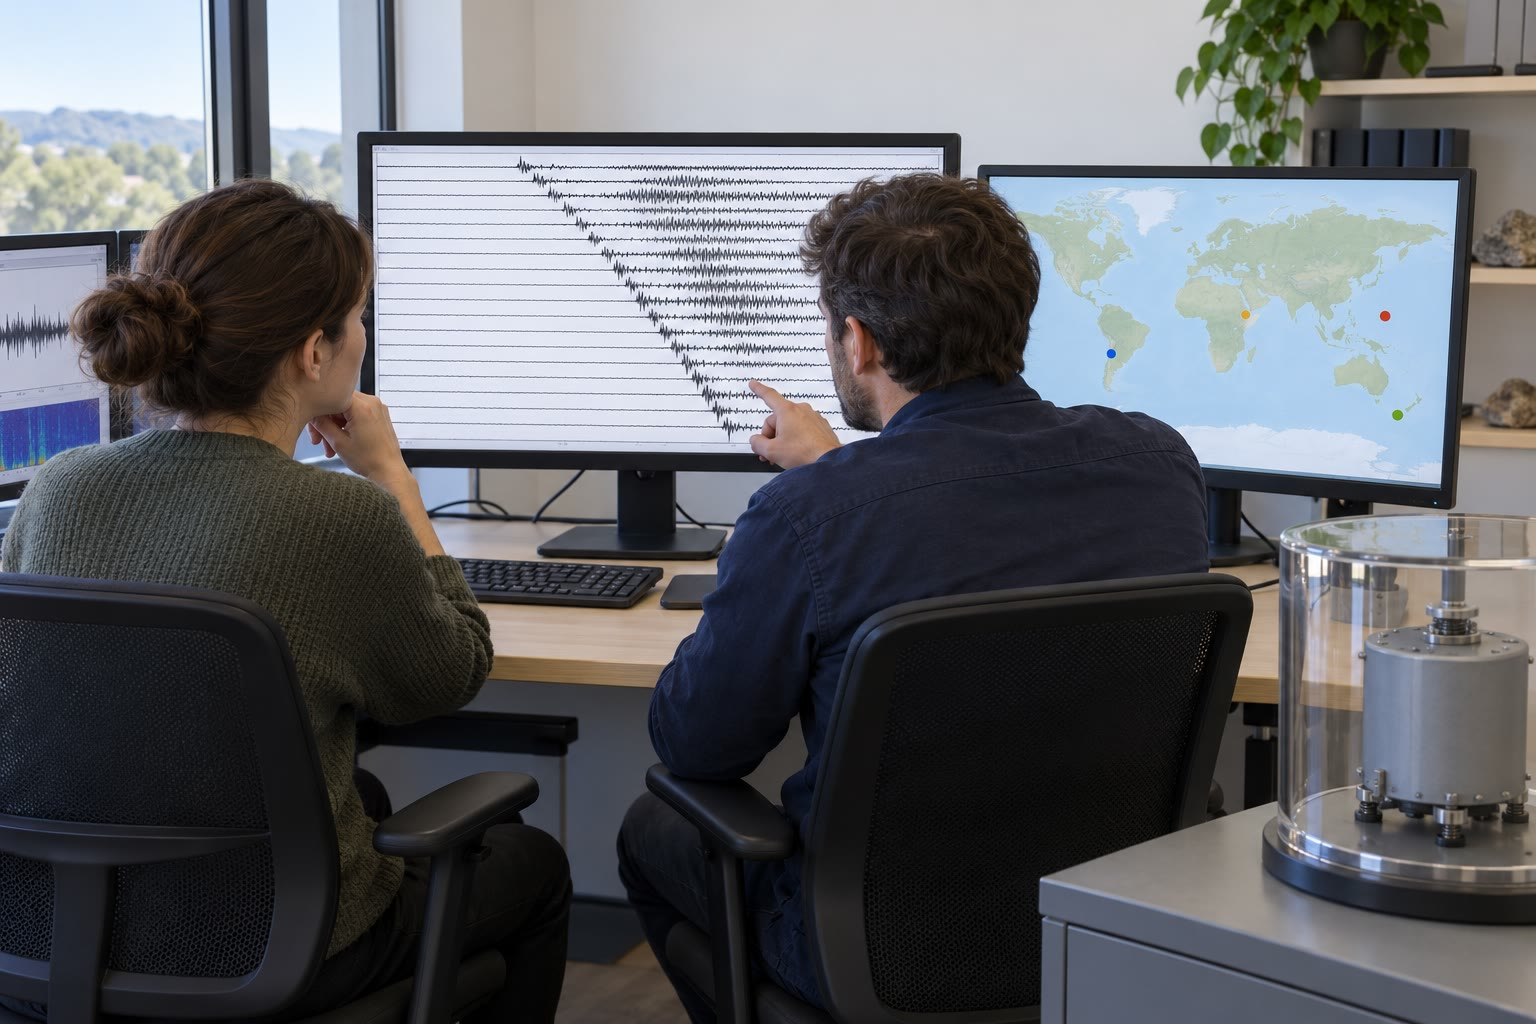
\includegraphics[width=\linewidth]{images/book3/ai/b1-seismic-analysis.jpg}

{\scriptsize 地震学家阅读记录剖面，同一次地震在各台站的记录道
按距离排列（AI 插图）。}
\end{minipage}
\end{inthelab}
% ledger: yvo:beachball

\section{测量加载：大地测量学}\label{sec:b1:earthquake-source:geodesy}

两次地震之间，锁定的断层对地震仪是不可见的，但
其周围的地面仍在移动。永久性卫星定位站测量这种
运动；各站速度穿过断层时的变化方式，可说明断层
被锁定的深度。

\begin{definition}[闭锁深度]\label{def:b1:earthquake-source:locking-depth}
断层的\emph{闭锁深度}\index{闭锁深度}，是指断层在两次地震之间被锁定的
深度；在此深度以下，断层以长期速率稳定滑动。
它是下一次地震中将发生滑动的那部分断层的
深度。
\end{definition}
% ledger: usgs:pp1515-thatcher

\begin{proposition}[穿越走滑断层的震间速度]\label{prop:b1:earthquake-source:interseismic}
设一条竖直的\omterm{def:b1:faults-folds-fabrics:fault-types}{走滑断层}位于弹性半空间中，自地表
至深度 $D$ 处被锁定，其下方以速率 $V$ 滑动。
距断层 $x$ 处、平行于断层的地表速度为
\[
  v(x) = \frac{V}{\pi}\arctan\frac{x}{D} .
\]
若断层在一次地震中滑动了 $s$（自地表至深度 $D$），
则地表位移为 $u(x) = (s/\pi)\arctan(D/x)$，其中 $x > 0$；
另一侧位移为 $-u(-x)$，其中 $x < 0$。
\end{proposition}
\admitted

该模型由 Savage 和 Burford 提出，是\omterm{def:b1:earthquake-source:seismic-cycle}{弹性
回跳}的最简形式，其曲线即第一幅图中围栏的曲线。其性质
可由公式直接导出。

\begin{proposition}[读取震间剖面]\label{prop:b1:earthquake-source:profile}
在\cref{prop:b1:earthquake-source:interseismic}的模型中：
\begin{enumerate}[label=(\alph*)]
  \item 远离断层时，速度趋于 $\pm V/2$，两侧板块
        以 $V$ 的相对速度运动；
  \item 速度在断层两侧的变化有一半发生在距断层
        $D$ 的范围内：$v(\pm D) = \pm V/4$；
  \item 地表的\omterm{def:b1:stress-strain-rheology:strain}{剪应变}速率 $\mathrm dv/\mathrm dx$ 在
        断层上最大，其值为 $V/(\pi D)$；
  \item 若断层在加载时间 $t$ 后于一次地震中滑动了 $s = Vt$，
        则地面最终在断层两侧各处分别发生 $\pm s/2$ 的位移，
        这一循环不留下永久弯曲，仅在断层上留下
        错动 $s$。
\end{enumerate}
\end{proposition}

\begin{proof}
(a) $\arctan(x/D) \to \pm\pi/2$，当 $x \to \pm\infty$ 时。(b) $\arctan 1 = \pi/4$，
故 $v(D) = V/4$，且 $v$ 为奇函数。(c) $\mathrm dv/\mathrm dx = (V/\pi D)/(1 +
x^2/D^2)$，在 $x = 0$ 处最大。(d) 当 $x > 0$ 时，加载使地面移动了
$t\,v(x) = (s/\pi)\arctan(x/D)$，地震则使其移动了
$(s/\pi)\arctan(D/x)$；由于 $\arctan y + \arctan(1/y) = \pi/2$（$y > 0$），
二者之和为 $s/2$。$x < 0$ 时符号相反，结论同样成立。
\end{proof}

性质 (b) 可由一组台站的剖面给出\omterm{def:b1:earthquake-source:locking-depth}{闭锁深度}：它是
距断层这样一段距离，在此处速度相对断层上的值
改变了 $V$ 的四分之一。浅闭锁使应变集中在
断层附近（见下图），深闭锁则使应变分布在较宽的
带状区域内。沿圣安德烈亚斯断层系，大地测量得到的\omterm{def:b1:earthquake-source:locking-depth}{闭锁深度}
在蠕滑段接近 0，最深可达 \qty{26}{km}，并与地震的深度相符：
被锁定的部分即
在\cref{ch:b1:stress-strain-rheology}中所述的\omterm{def:b1:stress-strain-rheology:strength-envelope}{孕震层}。取滑动速率为
\qty{34}{mm.\text{年}^{-1}}，\omterm{def:b1:earthquake-source:locking-depth}{闭锁深度}为 \qty{15}{km}，则断层上的\omterm{def:b1:stress-strain-rheology:strain}{剪应变}速率
为 $\num{0.034}/(\pi\times\num{15000}) = \num{7.2e-7}$ 每年，
这使一条横跨断层的直线每年弯曲不到每千米一毫米，
但在两个世纪内积累的数米错动，足以
引发一次大地震。
% ledger: sk:mu-locking, usgs:pp1515-wallace, usgs:pp1515-thatcher

\begin{omfigure}
\begin{tikzpicture}[font=\small]
\begin{axis}[omrecord, width=11cm, height=5.6cm, xmin=-100, xmax=100, ymin=-19, ymax=19,
    xlabel={距断层距离 $x$ (km)}, ylabel={速度 $v$ (\unit{mm.\text{年}^{-1}})},
    legend style={font=\scriptsize, at={(0.02,0.96)}, anchor=north west}, legend cell align=left]
  \addplot[omDef, line width=0.9pt, dashed] table[x=x, y=v5] {figdata/out/bachelor-1-interseismic-profiles.dat};
  \addplot[omThm, line width=1.1pt] table[x=x, y=v15] {figdata/out/bachelor-1-interseismic-profiles.dat};
  \addplot[omProp, line width=0.9pt, dotted] table[x=x, y=v25] {figdata/out/bachelor-1-interseismic-profiles.dat};
  \legend{$D = \qty{5}{km}$, $D = \qty{15}{km}$, $D = \qty{25}{km}$}
  \draw[black!50, dashed] (axis cs:-100,17) -- (axis cs:100,17);
  \draw[black!50, dashed] (axis cs:-100,-17) -- (axis cs:100,-17);
  \node[anchor=north west, font=\scriptsize] at (axis cs:-30,17) {$+V/2$};
  \node[anchor=south west, font=\scriptsize] at (axis cs:30,-17) {$-V/2$};
  \draw[black!60] (axis cs:0,-19) -- (axis cs:0,19);
  \node[anchor=east, font=\scriptsize] at (axis cs:-1,5) {断层};
\end{axis}
\end{tikzpicture}
\par\smallskip{\small 平行于锁定\omterm{def:b1:faults-folds-fabrics:fault-types}{走滑断层}的地面速度
（相对于断层迹线），滑动速率 $V = \qty{34}{mm.\text{年}^{-1}}$，
与沃勒斯溪 处圣安德烈亚斯断层的速率一致，图中给出三种\omterm{def:b1:earthquake-source:locking-depth}{闭锁深度}
（\cref{prop:b1:earthquake-source:interseismic}）。闭锁越浅，
速度发生变化的带越窄。}
\label{fig:b1:earthquake-source:interseismic}
\end{omfigure}
% ledger: usgs:pp1515-wallace

卫星定位只在少数台站测量地面。雷达卫星
则可覆盖整个区域：同一地区的两幅雷达图像，取自同一
轨道、不同时刻，逐波比较，其相位差
便描绘出地面与卫星之间距离的变化，
逐点进行，点距约一百米，无需
事先布设台站网。第一幅此类图像反映的是 1992 年加州一次大地震，
它在一张图中展示了同震位移，并与
野外和测量所得的错动相符；该技术即雷达干涉测量，
属于本科三年级分册的内容。
% ledger: massonnet:1993

\section{频次：古登堡–里克特定律}\label{sec:b1:earthquake-source:gr}

小地震远比大地震常见，而且
呈现出极为规整的规律。

\begin{proposition}[古登堡–里克特定律]\label{prop:b1:earthquake-source:gutenberg-richter}
设 $N$ 为某一地区、某一时段内\index{古登堡–里克特定律}
震级至少为 $M$ 的地震个数，满足
\[
  \log_{10} N = a - bM ,
\]
对目录\omterm{def:b1:earthquake-source:b-value}{完整性震级}以上的每个 $M$，
常数 $a$ 与 $b$ 依地区而定；$b$ 在多数
活跃地区中接近 1。
\end{proposition}
\admitted
% ledger: fd:1993, gr:1944

该定律是观测的结果，由本诺·古登堡与查尔斯·里克特
于 1944 年针对加利福尼亚发表，此后在各地均被发现；目前尚无理论
能推导出它，也推不出 $b$ 的数值。
% ledger: gr:1944

\begin{definition}[b 值、完整性震级]\label{def:b1:earthquake-source:b-value}
某一地区\omterm{prop:b1:earthquake-source:gutenberg-richter}{古登堡–里克特定律}中的常数 $b$ 称为该地区的
\emph{b 值}\index{b 值}。目录的\emph{完整性
震级}\index{完整性震级}是指使目录能完整记录该地区、该时段内
每一次地震的最小震级。
\end{definition}

\omterm{def:b1:earthquake-source:b-value}{b 值}为 1 意味着震级每增加一个单位，地震数目便减少为原来的十分之一。
低于\omterm{def:b1:earthquake-source:b-value}{完整性震级}时，计数落在直线之下，原因是
小地震被记录它们的台站太少，无法定位：定律
似乎发生弯曲，因此 $b$ 须在\omterm{def:b1:earthquake-source:b-value}{完整性震级}以上测定。对整个地球，
按浅源、中源和深源地震分别统计，测得的数值
介于 0.72 与 1.34 之间，但不同目录、震级范围或方法之间
常相差 \qty{30}{\percent} 或更多：数值远离 1 时，首先
应核查目录。
% ledger: fd:1993

\begin{omfigure}
\begin{tikzpicture}[font=\small]
\begin{axis}[omrecord, width=6.4cm, height=5.8cm, ymode=log, xmin=5.8, xmax=9.3, ymin=0.01, ymax=300,
    xlabel={震级 $M$}, ylabel={每年震级 $\ge M$ 的地震数},
    log basis y=10, title={(a) 频次与震级}, title style={font=\small}]
  \addplot[omProp, line width=0.9pt, domain=5.8:9.3] table[x=M, y=rate] {figdata/out/bachelor-1-gutenberg_richter-fit.dat};
  \addplot[only marks, mark=*, mark size=1.3pt, omDef] table[x=M, y=rate] {figdata/out/bachelor-1-gutenberg_richter-counts.dat};
  \draw[black!50, dashed] (axis cs:7.5,0.01) -- (axis cs:7.5,300);
  \node[anchor=south west, font=\scriptsize, omProp] at (axis cs:8.45,0.5) {$b = 1.01$};
  \node[anchor=north west, font=\scriptsize, align=left] at (axis cs:7.55,200) {拟合区间 \\ $6.0 \le M \le 7.5$};
\end{axis}
\begin{axis}[omrecord, at={(7.6cm,0)}, width=6.4cm, height=5.8cm, xmin=5.8, xmax=9.3, ymin=0, ymax=1.05,
    xlabel={震级 $M$}, ylabel={震级 $\ge M$ 的地震所占地震矩份额},
    title={(b) 地震矩的去向}, title style={font=\small}]
  \addplot[const plot, omDef, line width=0.9pt] table[x=M, y=share] {figdata/out/bachelor-1-gutenberg_richter-moment.dat};
\end{axis}
\end{tikzpicture}
\par\smallskip{\small 全球震级 6 或以上的 \num{7031} 次地震，
1976--2025 年（美国地质调查局目录）。(a) 每年震级至少为 $M$ 的
地震数；直线为 $\log_{10} N$ 对 $M$ 的最小二乘拟合，
拟合区间为 6.0 至 7.5，各计数均超过 200：
$\log_{10} N = 8.20 - 1.01\,M$ 每年。震级 8 以上的少数地震
落在直线之下。(b) 震级不小于某一值的地震所释放的
\omterm{def:b1:earthquake-source:moment}{地震矩}占总量的份额，其中 $M$ 为震级下限，每次\omterm{def:b1:earthquake-source:moment}{地震矩}按
$10^{1.5M + 9.1}$\,\unit{N.m} 计算：震级 8 或以上的 40 次地震
释放了总量的 \qty{63}{\percent}。}
\label{fig:b1:earthquake-source:gutenberg-richter}
\end{omfigure}
% ledger: data:usgs-comcat (fit and shares computed in figdata/bachelor-1/gutenberg_richter.py)

对图中的全球目录，取 $a = 8.20$、$b = 1.01$ 的定律
预测每年震级 7 或以上的地震为 14 次，与观测相符；震级 8 或以上的
地震预测为 1.35 次，而五十年间记录到 40 次，即每年 0.8 次。是否
最大地震确实少于直线所示（断层的有限尺寸暗示如此），
抑或只是过于罕见，以致五十年中未曾出现，此点尚未能
由如此少的事件定论。目录中约九分之一的震级是
面波或体波震级，这类震级会饱和；最大的地震
全部采用\omterm{def:b1:earthquake-source:mw}{矩震级}。
% ledger: data:usgs-comcat

大量小地震对释放\omterm{def:b1:earthquake-source:moment}{地震矩}的贡献很小。震级每减小一个单位，其数目增加
十倍，但\omterm{def:b1:earthquake-source:moment}{地震矩}则缩小 31.6 倍。

\begin{proposition}[最大地震释放了大部分地震矩]\label{prop:b1:earthquake-source:largest}
设地震服从\omterm{prop:b1:earthquake-source:gutenberg-richter}{古登堡–里克特定律}，且 $b < 1.5$，直至
最大震级 $M_{\max}$，并将其按每档宽为一个震级单位分组，
最高一档止于 $M_{\max}$。则最高一档的地震
所释放的\omterm{def:b1:earthquake-source:moment}{地震矩}超过总量的 $1 - 10^{-(1.5 - b)}$ 这一比例，
无论所计的最小震级多小：
对 $b = 1$，超过 \qty{68}{\percent}。
\end{proposition}

\begin{proof}
将各档自最小一档起依次编号为 $k = 0, 1, \dots, K$，第 $k$ 档
自 $M_k$ 至 $M_k + 1$，且 $M_{k+1} = M_k + 1$。由定律，
第 $k$ 档中的地震数为 $10^{a - bM_k} - 10^{a - b(M_k+1)} =
10^{a - bM_k}(1 - 10^{-b})$；由\cref{prop:b1:earthquake-source:moment-steps}可知
每次地震的\omterm{def:b1:earthquake-source:moment}{地震矩}介于 $10^{1.5M_k + 9.1}$ 与其 $10^{1.5}$ 倍之间，
且由于每一档均为前一档平移一个单位，第 $k$ 档的
\omterm{def:b1:earthquake-source:moment}{地震矩}为 $C q^k$，其中 $C$ 为常数，公比
$q = 10^{-b}\times10^{1.5} = 10^{1.5 - b} > 1$。总和为等比级数
\[
  S = C(1 + q + \dots + q^K) = C\,\frac{q^{K+1} - 1}{q - 1} ,
\]
最高一档所占的份额为
\[
  \frac{C q^K}{S} = \frac{q^K (q - 1)}{q^{K+1} - 1}
  > \frac{q^K (q - 1)}{q^{K+1}} = 1 - \frac1q = 1 - 10^{-(1.5 - b)} .
\]
对 $b = 1$，$1 - 10^{-0.5} = 0.684$。
\end{proof}

在世界目录中，份额大致如此：最大一档震级
即震级 8.1 至 9.1 的那一档，五十年内释放了一半以上的\omterm{def:b1:earthquake-source:moment}{地震矩}，而
两次最大的地震，即 2004 年苏门答腊–安达曼地震与 2011 年东北地震，
震级均为 9.1，二者合计释放了 \qty{29}{\percent}。板块边界需释放的
\omterm{def:b1:earthquake-source:moment}{地震矩}由其滑动速率决定；命题断言，该\omterm{def:b1:earthquake-source:moment}{地震矩}几乎全部
在其最大的几次地震中释放，而大量小地震，尽管频繁发生，
并不能减轻断层对下一次大地震的负担。
% ledger: data:usgs-comcat, usgs:sumatra-mt, usgs:tohoku-mt

\section{练习}

\begin{exercise}[$\star$]\label{exo:b1:earthquake-source:1}
(a) 计算\omterm{def:b1:earthquake-source:moment}{地震矩}为
\qty{4e17}{N.m} 的地震的\omterm{def:b1:earthquake-source:mw}{矩震级}。(b) 东北地震的 $M_0 = \qty{5.59e22}{N.m}$，
请核对其震级。(c) 震级为
7.0 的地震，其\omterm{def:b1:earthquake-source:moment}{地震矩}是多少？
% ledger: usgs:tohoku-mt
\end{exercise}

\begin{exercise}[$\star$]\label{exo:b1:earthquake-source:2}
一条\omterm{def:b1:faults-folds-fabrics:fault-types}{走滑断层}以 \qty{25}{mm.\text{年}^{-1}} 的速率加载，其地震
每次错动约 \qty{3}{m}。(a) 若两次地震之间
断层完全闭锁，其\omterm{def:b1:earthquake-source:seismic-cycle}{复发间隔}为多少？(b) 若一半的滑动速率由
稳态蠕动承担，又如何？
\end{exercise}

\begin{exercise}[$\star$]\label{exo:b1:earthquake-source:3}
震级为 7.4 的地震的\omterm{def:b1:earthquake-source:moment}{地震矩}，是震级为
6.2 的地震的多少倍？需要多少个震级为
6.2 的地震才能释放相同的\omterm{def:b1:earthquake-source:moment}{地震矩}？
\end{exercise}

\begin{exercise}[$\star$]\label{exo:b1:earthquake-source:4}
在 $b = 1$ 的区域中，每年记录到一千次震级为 3 或以上的地震。
每年预计震级为 5 或以上、
震级为 6 或以上的地震各有多少次？
震级为 7 或以上的地震之间，平均间隔多久？
\end{exercise}

\begin{exercise}[$\star\star$]\label{exo:b1:earthquake-source:5}
1906 年的地震沿圣安德烈斯断层破裂了约 \qty{430}{km}。
(a) 设破裂深达 \qty{15}{km}，平均错动为
\qty{4}{m}，取 $\mu = \qty{30}{GPa}$，计算其\omterm{def:b1:earthquake-source:moment}{地震矩}与
\omterm{def:b1:earthquake-source:mw}{矩震级}。(b) 若破裂仅深达
\qty{10}{km}，震级变化多少？(c) 两种估计中，哪一个更接近 7.9？
% ledger: pp1515:1906, usgs:hist-mw
\end{exercise}

\begin{exercise}[$\star\star$]\label{exo:b1:earthquake-source:6}
东北地震的破裂长约 \qty{400}{km}，
宽约 \qty{150}{km}，\omterm{def:b1:earthquake-source:moment}{地震矩}为 \qty{5.59e22}{N.m}。(a) 取 $\mu = \qty{30}{GPa}$，计算其
平均错动量。(b) 太平洋板块以约
\qty{83}{mm.\text{年}^{-1}} 的速率俯冲于日本之下，若界面完全闭锁，
积累此错动量需多长时间？(c) 若闭锁比例为 0.8，
或 0.5，又各需多长时间？
% ledger: usgs:tohoku-mt, usgs:tohoku-summary
\end{exercise}

\begin{exercise}[$\star\star$]\label{exo:b1:earthquake-source:7}
2004 年苏门答腊–安达曼地震的一个\omterm{def:b1:earthquake-source:focal-mechanism}{节面}\omterm{def:b1:geological-maps:attitude}{走向}为 $329$，\omterm{def:b1:geological-maps:attitude}{倾角}
\ang{8}，\omterm{def:b1:faults-folds-fabrics:fault-elements}{侧伏角} \ang{110}。(a) 以东、北、
上分量写出 $\mathbf n$ 与 $\mathbf d$。(b) 求\omterm{def:b1:earthquake-source:focal-mechanism}{辅助面}的\omterm{def:b1:geological-maps:attitude}{走向}、\omterm{def:b1:geological-maps:attitude}{倾角}与\omterm{def:b1:faults-folds-fabrics:fault-elements}{侧伏角}。
(c) 求 \omterm{def:b1:earthquake-source:focal-mechanism}{P 轴}与 \omterm{def:b1:earthquake-source:focal-mechanism}{T 轴}的\omterm{def:b1:field-lab-methods-1:trend-plunge}{倾伏向}和\omterm{def:b1:field-lab-methods-1:trend-plunge}{倾伏角}。(d) 哪一个\omterm{def:b1:earthquake-source:focal-mechanism}{节面}是
断层面，该断层属于何种类型？
% ledger: usgs:sumatra-mt
\end{exercise}

\begin{exercise}[$\star\star$]\label{exo:b1:earthquake-source:8}
\omterm{def:b1:geological-maps:attitude}{走向}为 $045$ 的竖直断层发生\omterm{def:b1:faults-folds-fabrics:fault-types}{右行}错动。(a) 对于从震源
水平射向正北、正东、正南、正西方向的台站的波，哪些以压缩
到达、哪些以拉张到达？(b) 给出 \omterm{def:b1:earthquake-source:focal-mechanism}{P 轴}与 \omterm{def:b1:earthquake-source:focal-mechanism}{T 轴}的\omterm{def:b1:field-lab-methods-1:trend-plunge}{倾伏向}。(c) 证明
对\omterm{def:b1:geological-maps:attitude}{走向}为 $135$ 的竖直面上的\omterm{def:b1:faults-folds-fabrics:fault-types}{左行}错动，同样给出
相同的\omterm{def:b1:earthquake-source:focal-mechanism}{初动}分布。
\end{exercise}

\begin{exercise}[$\star\star$]\label{exo:b1:earthquake-source:9}
穿越一条闭锁\omterm{def:b1:faults-folds-fabrics:fault-types}{走滑断层}，两侧的远场台站相对运动，
相对速率为 \qty{40}{mm.\text{年}^{-1}}。距断层 \qty{10}{km} 的一个台站
相对断层迹线以 \qty{10}{mm.\text{年}^{-1}} 的速度运动。(a) 求
\omterm{def:b1:earthquake-source:locking-depth}{闭锁深度}。(b) 预测距断层
\qty{30}{km} 处台站的速度。(c) 计算断层上的\omterm{def:b1:stress-strain-rheology:strain}{剪应变}速率。
\end{exercise}

\begin{exercise}[$\star\star\star$]\label{exo:b1:earthquake-source:10}
(a) 证明：若 $b$ 大于 1.5，则区域内地震的总\omterm{def:b1:earthquake-source:moment}{地震矩}
将由最小的地震主导。(b) 对于 $b = 0.8$，最大一档震级
至少释放多大比例的\omterm{def:b1:earthquake-source:moment}{地震矩}？(c) 若采用世界目录的
$a = 8.20$ 与 $b = 1.01$（每年），按该定律预测五十年内将出现多少次
震级为 9 或以上的地震？该目录在 1976–2025 年间
仅记录到两次，试作评论。
% ledger: data:usgs-comcat
\end{exercise}

\begin{exercise}[$\star\star\star$]\label{exo:b1:earthquake-source:11}
一道直线栅栏横跨一条闭锁\omterm{def:b1:faults-folds-fabrics:fault-types}{右行}断层，其中 $V =
\qty{34}{mm.\text{年}^{-1}}$，$D = \qty{15}{km}$。(a) 经过 150 年，
距断层以东 \qty{1}{km}、\qty{15}{km} 与 \qty{50}{km} 处的立柱，
相对于断层上的立柱，沿断层移动了多少？(b) 随后断层在一次地震中
滑动全部亏损量。求此错动量，以及三根立柱各自在地震中移动了多少？
三根立柱在地震中各移动了多少？(c) 用三根立柱检验
\cref{prop:b1:earthquake-source:profile} 的 (d) 部分。
% ledger: usgs:pp1515-wallace
\end{exercise}

\begin{exercise}[$\star\star\star$]\label{exo:b1:earthquake-source:12}
某地震的水平 \omterm{def:b1:earthquake-source:focal-mechanism}{P 轴}\omterm{def:b1:field-lab-methods-1:trend-plunge}{倾伏向}为 $000$，水平 \omterm{def:b1:earthquake-source:focal-mechanism}{T 轴}
\omterm{def:b1:field-lab-methods-1:trend-plunge}{倾伏向}为 $090$。(a) 证明其\omterm{def:b1:earthquake-source:focal-mechanism}{节面}为竖直面，\omterm{def:b1:geological-maps:attitude}{走向}分别为 $045$
与 $135$，并利用 $\mathbf n$、$\mathbf d = (\mathbf T \pm \mathbf P)/\sqrt2$。
(b) 给出每个\omterm{def:b1:earthquake-source:focal-mechanism}{节面}上的错动方向。(c) 若断层是在岩石中新形成的，
在\omterm{def:b1:stress-strain-rheology:coulomb}{内摩擦角}为 $\phi = \ang{30}$ 的岩石中、沿 \omterm{def:b1:earthquake-source:focal-mechanism}{P 轴}方向的 $\sigma_1$ 作用下，
它将位于哪些\omterm{def:b1:geological-maps:attitude}{走向}上？为何 \omterm{def:b1:earthquake-source:focal-mechanism}{P 轴}只是
$\sigma_1$ 的近似？(d) 附近一条已测绘的断层\omterm{def:b1:geological-maps:attitude}{走向}为 $040$，哪一个\omterm{def:b1:earthquake-source:focal-mechanism}{节面}
很可能是该断层？其错动方向如何？
\end{exercise}

\section{问题：锁定断层上的下一次大地震}

\begin{problem}[{周末问题——走滑板块边界上的锁定段，
从其加载、既往地震，直到下一次地震的震级
}]
\label{pb:b1:earthquake-source:1}
% values: calc/ch18.py; an invented fault (the numbers are of a realistic order)
一条笔直的竖直\omterm{def:b1:faults-folds-fabrics:fault-types}{走滑断层}构成两个板块之间的边界。
其中一段长 \qty{250}{km}，处于锁定状态，其地震的起始深度
不超过 \qty{15}{km}。横跨断层开挖的探槽将其最近四次大地震
定年为约 1050、1290、1480 和 1712 年，位移分别为 \num{7.0}、
\num{6.0}、\num{5.5} 和 \qty{7.5}{m}。远离断层、位于断层两侧的
永久台站相对移动速率为 \qty{30}{mm.\text{年}^{-1}}。取 $\mu =
\qty{30}{GPa}$，以 2025 年为现在，并给出震级，精确到 0.01。

\medskip
\noindent\textbf{第一部分——加载。}
\begin{enumerate}
  \item 计算四次地震之间的间隔及其平均值。
  \item 计算平均位移，并利用
        \cref{prop:b1:earthquake-source:recurrence}求出完全锁定断层的\omterm{def:b1:earthquake-source:seismic-cycle}{复发间隔}。
  \item 仅由探槽资料计算滑动速率：取最后三次地震的位移，
        以及这三次中首次与末次地震之间的时间。
        并与大地测量速率比较。
  \item 最近一次地震距今多久？若该段完全锁定，
        自那以来累积了多少滑动亏损？
  \item 将此亏损与探槽中的位移比较。下一次
        地震是否已超期？
  \item 为何探槽无法给出下一次地震的日期？
\end{enumerate}

\medskip
\noindent\textbf{第二部分——下一次地震的大小。}
\begin{enumerate}[resume]
  \item 该段锁定部分的面积是多少？
  \item 计算能释放全部亏损的一次地震的
        \omterm{def:b1:earthquake-source:moment}{地震矩}。
  \item 假定 1712 年地震破裂的面积相同，并取探槽位移为平均滑动量，
        计算该次地震的\omterm{def:b1:earthquake-source:mw}{矩震级}。
  \item 下一次地震的\omterm{def:b1:earthquake-source:moment}{地震矩}超过 1712 年地震的
        多少倍？这相当于\omterm{def:b1:earthquake-source:mw}{矩震级}相差多少个单位？
  \item 若只有该段的一半破裂，且滑动量相同，
        其震级将为多少？
  \item 给出该段每年积累的\omterm{def:b1:earthquake-source:moment}{地震矩}。
\end{enumerate}

\medskip
\noindent\textbf{第三部分——频度与能量。}
\begin{enumerate}[resume]
  \item 区域目录遵循 $\log_{10} N = 4.3 - M$（每年），
        由该区域所有断层的地震给出。其 \omterm{def:b1:earthquake-source:b-value}{b 值}为多少？
        每年给出多少次震级 5 级或以上的地震，
        以及多少次 6 级或以上的地震？
  \item 据此目录，震级 7 级或以上的地震的平均间隔时间为多少，
        震级 8 级或以上的呢？
  \item 比较由目录得到的大地震\omterm{def:b1:earthquake-source:seismic-cycle}{复发间隔}与
        由探槽得到的\omterm{def:b1:earthquake-source:seismic-cycle}{复发间隔}。这一差异对用小地震的
        规律预测大地震说明了什么？
  \item 区域规律中震级 5 至 8 级的地震，合计
        每年释放约 \qty{5.5e17}{N.m}。这占该段\omterm{def:b1:earthquake-source:moment}{地震矩}的
        多大比例？
  \item 下一次大地震辐射的能量是震级 6 级地震的
        多少倍？
  \item 利用\cref{prop:b1:earthquake-source:largest}，说明该段的中等地震
        为何不能缓解它。
\end{enumerate}

\medskip
\noindent\textbf{第四部分——由台站求锁定深度。}
\begin{enumerate}[resume]
  \item 穿过该段的一条台站剖面给出，相对于断层迹线的
        速度为 $-11.6$、$-7.5$、$-3.1$、$3.1$、$7.5$ 及
        \qty{11.6}{mm.\text{年}^{-1}}，位置为 $x = -40$、$-15$、$-5$、$5$、$15$ 及
        \qty{40}{km}处。检验该剖面是否反对称，并给出
        远离断层处的预期速度。
  \item 由位于 \qty{15}{km} 处的台站，计算\omterm{def:b1:earthquake-source:locking-depth}{闭锁深度}。
  \item 再由位于 \qty{5}{km} 和 \qty{40}{km} 处的台站计算一次，并
        解释两者之间的微小差异。
  \item 将\omterm{def:b1:earthquake-source:locking-depth}{闭锁深度}与地震的深度比较，并说明
        二者为何应当一致。
  \item 计算断层上的\omterm{def:b1:stress-strain-rheology:strain}{剪应变}率。
  \item 精确到 0.01，能释放该段全部滑动亏损的
        地震的\omterm{def:b1:earthquake-source:mw}{矩震级}是多少？
\end{enumerate}
\end{problem}
